\chapter{I Had \$78\ldots\ Now I'm Worth \$100 Million}

This interview contains almost no formal blackboard mathematics, but it does have a clear quantitative spine. We move from spectacle to thresholds: a private jet with a real operating burden, a tail number that encodes a former balance of \$78, a sleep-testing business that scales from a kitchen desk to more than a million tested patients, and a closing rule of thumb that private aviation belongs only after disposable income clears a recurring cash-flow floor. The lecture is therefore best read as a study in commercial arithmetic, operating constraints, and leverage.

\section{Jet, Tail Number, and the Arithmetic of Proof}

The lecture opens with a familiar image and then immediately attacks the image. We begin with the jet because that is what the eye sees; we remain with the jet because the speaker insists that it cannot be treated as decoration. A car can be rented, borrowed, or staged. A plane, by contrast, has to be carried.

The first quantitative claims are blunt:
\begin{align}
4 &\mapsto \text{April}, &
78 &\mapsto \$78, \\
C_{\text{jet}} &> \$5\,\text{million}, &
O_{\text{jet,yr}} &\approx \$2\,\text{million/year}.
\end{align}
The first line is symbolic rather than financial. The tail number is not a formula for wealth; it is a compressed autobiographical marker. The second line is the real point. The jet becomes an operating object, and once that happens the lecture ceases to be about status and becomes a lecture about thresholds.

A useful example is built into the interview itself. Suppose the jet were somehow free. Then the acquisition burden disappears, but the lecture claims the recurring burden remains:
\begin{align}
C_{\text{jet}} &\to 0, \\
O_{\text{jet,yr}} &\approx \$2\,\text{million/year}.
\end{align}
So even in the gift case the asset still demands a stream of cash. This is the first clean derivation in the interview: ownership is not defined by purchase alone; it is defined by the ability to absorb recurring cost.

The host briefly resets the story by narrating his own flight from Miami to Tampa. That reset matters. The plane is not merely discussed; it changes who can be interviewed, where, and under what conditions. Access is already entering the story.

\section{From \$78 to Commitment}

Once the tail number has been decoded, the lecture asks its first real question: what is the first actionable step when one is down to \$78?

\subsection{Question \& Answer}

\paragraph{Question.} What is the first actionable step when you are nearly broke?

\paragraph{Answer.} The answer is not a tactic. It is commitment. The speaker does not present commitment as enthusiasm, or as one priority among many, but as a reordering in which the business goal becomes dominant over comfort, sleep, and convenience.

This is important for the notes because the lecture is careful here. It does not pretend that cash appears from willpower alone. Rather, it says that before any mechanism can work, the entrepreneur must stop treating the project as optional. In the logic of the interview, the first threshold is not financial but existential.

What follows immediately after this answer is also important. The speaker is asked whether the sacrifice was worth it, and he answers yes in two currencies at once: money and quality of life. He mentions the ability to fly to Medell\'{\i}n, to maintain an office and a house there, and to manage a workforce of roughly \(350\) employees in that city. So the lecture’s first payoff is not merely symbolic redemption but operating range.

\section{A Niche Healthcare Machine}

Only after the commitment question has been answered do we learn what the business actually is. This ordering matters. The lecture does not begin with market selection in the abstract; it first fixes seriousness, and only then shows us the domain in which seriousness is applied.

The business is Blackstone Medical Services, described as the largest provider of medical sleep testing in the United States. The scale claims are concrete:
\begin{equation}
N_{\text{emp}} > 650, \qquad N_{\text{pat}} > 10^6.
\end{equation}
We are also given a timeline anchor:
\begin{equation}
t_{\text{start}} = 2012.
\end{equation}
The speaker says that the company began in his kitchen, that early volume was only a couple of hundred patients per month, and that by May of the current year the cumulative tested-patient count had crossed one million.

The pedagogical point is that the business is not glamorous in the usual startup sense. It is narrow, institutional, and service-heavy. That is precisely why it matters. The lecture is pushing us away from the fantasy that wealth must begin with a dazzling product category. Here wealth begins in a medical niche, with repeated testing, institutional relationships, and scale through reliability.

The second point is motivational rather than sentimental. The speaker insists that passion matters because without it one abandons the project at the first serious friction. We should state that carefully. The lecture does not mean that passion substitutes for execution. It means that passion keeps execution alive long enough for execution to matter.

\section{Sleep as an Operating Constraint}

The subject of the company now folds back onto the life of the operator. Because the business lives in sleep medicine, the host asks whether sleep actually matters for success. The answer is one of the sharpest small claims in the interview: sleep is not a moral weakness, and it is not a luxury. It is an input into cognition.

The speaker’s threshold is stated plainly:
\begin{align}
h_{\text{sleep}} &\in [6,7]\ \text{hours/night}, \\
h_{\text{sleep}} < h_{\min} &\Rightarrow \text{drag, weaker attention, poorer focus}.
\end{align}
This is not a laboratory law. It is a personal operating law. But the lecture wants us to take it seriously because entrepreneurship is described here as a long-duration attention problem. If the day runs to \(12\), \(13\), or \(14\) hours, then degraded attention is not a detail; it is a direct business cost.

\subsection{Question \& Answer}

\paragraph{Question.} Does sleep actually matter for entrepreneurial performance, or is sleep deprivation part of the myth?

\paragraph{Answer.} In the lecture, sleep matters because business work is cognitive work. Meetings, focus, memory, judgment, and sustained attention all degrade once the sleep threshold is crossed downward. The myth that sleep is for weak people is rejected outright.

The order is again deliberate. We move from the niche to the body, and then from the body back down to the actual mechanics of starting the firm.

\section{Kitchen Start and the Market Funnel}

Now we are finally taken into the small machinery of the beginning. The speaker describes pajamas, a white desk, an Apple computer, a recent divorce, two young children, and the sense of starting over. One could sentimentalize this; the lecture does not. It becomes interesting only when it becomes operational.

The first operational fact is that the United States is described as an insured market:
\begin{equation}
r_{\text{insured}} \approx 0.97.
\end{equation}
That claim motivates the first half of the funnel: insurer contracts. The second half is doctor acquisition. Each morning begins with emails to insurance companies; the day continues with calls on doctors to win business. The point is not that either leg alone is sufficient. The point is that patient volume is downstream of both.

A compact reconstruction is
\begin{equation}
F_{\text{patients}} = F(C_{\text{ins}},D_{\text{doc}}),
\end{equation}
where \(C_{\text{ins}}\) denotes insurer contracting and \(D_{\text{doc}}\) denotes physician-side business development. This is only a schematic relation; the interview gives no conversion rates. But the schematic relation is worth preserving because it shows that the origin story hides a two-channel acquisition system.

The first office is also quantified:
\begin{equation}
R_{\text{office}} = \$500/\text{month}, \qquad A_{\text{office}} \approx 500\ \text{ft}^2.
\end{equation}
That small office matters for the same reason the \$78 matters. The lecture repeatedly wants a story to crystallize into a number.

\begin{figure}
\centering
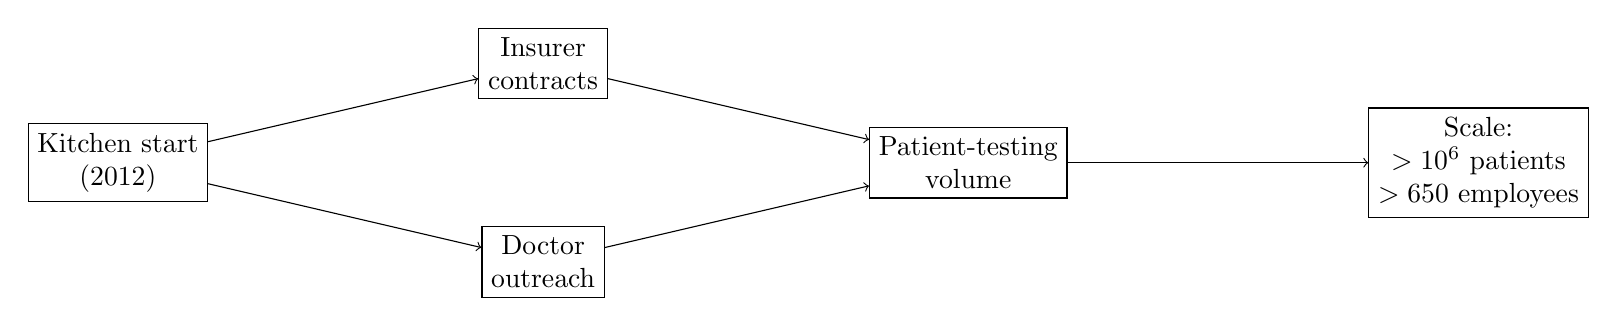
\begin{tikzpicture}[x=2.7cm,y=1.4cm]
\node[draw, rectangle, align=center] (k) at (0,0) {Kitchen start\\(2012)};
\node[draw, rectangle, align=center] (i) at (2,0.9) {Insurer\\contracts};
\node[draw, rectangle, align=center] (d) at (2,-0.9) {Doctor\\outreach};
\node[draw, rectangle, align=center] (p) at (4,0) {Patient-testing\\volume};
\node[draw, rectangle, align=center] (s) at (6.4,0) {Scale:\\\(>10^6\) patients\\\(>650\) employees};
\draw[->] (k) -- (i);
\draw[->] (k) -- (d);
\draw[->] (i) -- (p);
\draw[->] (d) -- (p);
\draw[->] (p) -- (s);
\end{tikzpicture}
\caption{A schematic reconstruction of the startup funnel described in the interview.}
\end{figure}

This figure is not a hidden board derivation. It is a clean way of preserving the sequence that the lecture describes verbally.

\section{Service, Team, and Bankability}

The lecture now asks what made the business win. The answer is not product alone. Other products exist. The differentiator is the service layer wrapped around the product. In a cautious reconstruction we may write
\begin{equation}
Q_{\text{offer}} = Q_{\text{product}} + Q_{\text{service}},
\end{equation}
provided we remember that this is a note-writer’s compression, not the speaker’s literal algebra.

The scale claim that follows is striking:
\begin{equation}
\Delta W_{3\text{--}4\text{ yr}} \approx \$85\,\text{million}.
\end{equation}
The explanation is equally striking: the move-the-needle factor is team investment. There was even a period in which employees made more money than the founder, precisely because the founder chose to invest into scale.

This gives us a second compact structural claim:
\begin{equation}
N_{\text{emp}} \gg 1 \quad \Rightarrow \quad Y_{\text{firm}} \not\approx Y_{\text{founder-alone}}.
\end{equation}
The point is not to demote the founder. In fact the speaker insists that the founder remains the most important person in the company. The point is rather that importance and throughput are different notions. Importance may stay concentrated, while throughput must become distributed.

\subsection{Question \& Answer}

\paragraph{Question.} What actually moves the needle when a founder can no longer do everything alone?

\paragraph{Answer.} The lecture’s answer is team leverage. Product matters, but the business becomes scalable only when the founder pays for capability in others, accepts that some of them may be better compensated, and stops pretending that a \(650\)-person enterprise can be run by personality alone.

From here the lecture becomes more infrastructural. Three roles are singled out: accountant, operations lead, and CTO. Their order is meaningful. Accounting comes first because bankability comes before elegance. The lecture’s logic is
\begin{equation}
\text{clean books} \Rightarrow B_{\text{bankable}} \Rightarrow \text{credit access and sale readiness}.
\end{equation}
The operations lead is the person in the weeds. The CTO is the one asked to think forward in a \(3\)-to-\(5\)-year horizon. So the business is now being described not as hustle in the air but as an institution with bookkeeping, execution, and technical direction.

There is a brief inserted interlude in which the host repeats a bookkeeping maxim: know your numbers better than your product. We do not need the surrounding advertisement. The durable point is already consistent with the interview itself.

\section{Shrewdness, Negotiation, Competition, and Access}

The late part of the lecture shifts from how the firm was built to how an operator must think. The speaker describes himself as a student, insists that one is finished the moment one thinks one knows everything, and then offers a series of doctrines: shrewdness, cost realism, the refusal to name the first number in a negotiation, competitive consistency, and investment in access.

The most memorable anecdote concerns bagels and coffee. A wealthy mentor refuses an inflated charge on a jet not because he cannot pay it, but because the line item does not correspond to what the thing actually costs. The lesson is beautifully simple: luxury does not repeal arithmetic.

The competition story is equally concrete. The industry is said to have contained large incumbents. A major competitor was still alive in 2018, but around 2019 the speaker claims to have surpassed that competitor in volume and to have remained the largest player since then. The mechanism given is not secret technology. It is consistency: deliver, deliver, deliver, with no room for error when thousands of patients are moving through the system daily.

Negotiation is treated in the same spirit. One should not give the first number. If we let \(a_1\) denote the first anchor in a negotiation, then the lecture’s practical rule is
\begin{equation}
\text{do not set } a_1 \text{ first.}
\end{equation}
The reasoning is standard: the first anchor reveals information before the other side has exposed its range. The lecture does not need game theory to make the point, because the point is already clear from experience.

A final threshold metaphor closes this entire cluster: water boils at \(212\), not \(211\). We should not literalize the metaphor. Its purpose is to say that late-stage advantage may look numerically small and yet be decisively consequential.

\subsection{Question \& Answer}

\paragraph{Question.} How much money do you actually need before a private jet is a business asset rather than a fantasy prop?

\paragraph{Answer.} The lecture gives a practical floor:
\begin{align}
I_{\text{disp}} &\in [\$2,\$3]\,\text{million/year}, \\
I_{\text{disp}} &\gtrsim O_{\text{jet,yr}}.
\end{align}
The important idea is that the plane only becomes intelligible once it is downstream of business cash flow. By that stage it is not merely transport. It is an amplifier of convenience, family mobility, mentor access, and high-value conversation. The host asks whether the speaker networks with more billionaires since buying the plane, and the answer is yes. So the object with which the lecture began returns at the end, but now it has changed category. It is no longer spectacle. It is a network machine purchased after a threshold has been crossed.

\section{Summary}

The chapter begins with a jet and ends with a threshold. In between, the lecture builds a chain of operating constraints: a tail number that remembers \$78, commitment before tactics, a healthcare niche rather than a glamorous startup, sleep as a cognitive floor, a two-channel acquisition funnel, service as differentiator, team as leverage, accounting as the precondition of bankability, shrewdness in cost and negotiation, and finally the reappearance of the jet as a consequence rather than a premise. That is the real mathematics of the interview: not formal theory, but disciplined relations among cost, focus, scale, and proof.